\chapter{需求分析}
\label{chap:requirements-analysis}

\section{总体需求}
在上一章绪论中,我们已经提到目前有大量的病历数据并没有电子化,或无法与现有的电子病历系统兼容协同,我们称之为未归档数据。从形成原因来说,未归档数据大致可以分为两大类:
\begin{itemize}
	\item 病历电子化之前的纸质档案,即现在很多医院的病历系统已经电子化,但是电子化之前的病历档案数据,仍然是纸质化的,这部分档案数据量庞大,包含了病人的历史诊疗记录,在临床上有很高的参考利用价值,故不能轻易舍弃,另一方面,旧的病历数据又很难与已有的电子化病历数据很好的协同使用,两者在档案产生、存储管理、信息展示、诊疗协助等各方面都有明显不同,为医院的诊疗工作进行提供了一些客观上的不便。
	\item 旧电子化系统中的档案,即一些医院存在着将旧的电子化病历系统废弃,采用新的电子化病历系统的情况,旧系统虽然废弃了,但是其保存的病人诊疗数据却是要保留和利用的。旧电子病历系统数据与纸质数据类似,也存在着与新电子化病历系统的协同问题,因此,如何将数据从旧系统向新系统迁移也是一个摆在面前的现实问题。
\end{itemize}
我们可以设想两个模拟的场景:
\begin{itemize}
	\item[场景A] 当一个病人去医院看病时,医生一边询问病人的主诉和症状,一边让助手去档案库中去找这个病人的过往诊疗记录,一边还要看医院电子档案系统的有关该病人的记录,纸质档案的寻找和放回都耗时耗力,面对等候在门外的患者长龙,医生可能只好根据已有的病人电子档案进行迅速诊断,这样势必会影响病人病情的综合判断。
	\item[场景B] 同样是一个病人来医院看病,医生询问病人的主诉和症状,一边的助手则根据已经录入到电子档案系统中的病人过往诊疗记录,适当提取相关信息,医生据此做出综合判断,迅速的确定病人的病情,给出来合理的治疗方案,整个过程高效且病情诊断可靠性高,病人有望迅速康复。
\end{itemize}
对比而言,场景A无疑是效率低下的,更严重是有可能影响病人病情的正确诊断,场景B则是医院的理想诊断过程,不仅效率高,且诊断更加全面准确。因此,如何将纸质病历数据和旧电子病历系统的数据迁移到新的电子化的病历系统中,是存在着广泛需求的,如果能够较好的解决这个问题,将能有效的改善现有医院病历系统的混乱现状,补全病人的医疗信息,提高诊疗效率,能给医院带来实际的效益。

\section{具体应用}
上一段中我们从总体上分析了病历档案生成与分类在医学领域的迫切需求和研究意义,现在我们更加细致的考虑这个问题,从系统角度来看,需求分析可以分别从系统环境、输入数据、输出数据以及性能这四个方面来论述。

\subsection{系统环境}
总体上,我们需要设计和实现一个病历档案生成和分类系统,系统在什么环境下运行呢?从成本、性能和稳定性等方面来综合考虑,这个系统的运行环境应该满足以下要求:
\begin{itemize}
	\item 系统能运行在普通的个人电脑上。这主要是出于成本的考虑,首先,个人电脑现在相当普及,易于获得,但是普遍性能较弱,稳定性没有保障。所以,系统应该能正常运行在性能较弱的个人电脑上。
	\item 系统能运行在商用服务器上。这主要是出于性能和稳定性上的考虑,服务器相对于个人电脑,性能更加强劲,同时,服务器有着高度的稳定性,整个系统可以很好的在服务器上长期稳定运行,持续产出,同时,服务器的一些特性也比较方便运维人员的维护和管理。
	\item 系统能对多种平台进行支持。医院内部采用的电子化系统可能运行在不同的平台上,对于主流平台,即Windows和Linux,以及Windows Server和Linux Server,系统都应该能够支持。同时,对于这些平台的不同版本(例如Windows 7和Windows XP),也要有较好的支持。
\end{itemize}

\subsection{输入数据}
\subsubsection{数据转换}
在这一章的开头,我们提到,待归档的数据主要有两类,纸质病历数据和旧电子化档案。在实际应用中,这两种数据都是不能直接被计算机系统识别的,因此,我们分别对其进行一定的转化:
\begin{itemize}
	\item 对于纸质数据,通过一台扫描仪或者照相机对病历进行录入,转换成图片数据。
	\item 对于旧电子化档案数据,我们可以在个人电脑上通过批处理的方式,打开旧电子病历,并利用个人电脑的截图功能,将病历转换成图片数据。
\end{itemize}
经过这样的转换后,这两种数据都已经转换成了图片数据,单个病人的病历诊疗数据,被转换成了多张图片数据保存下来。据此可以做进一步的处理。

\subsubsection{数据详解}
经过数据转换以后的图片数据长什么样呢,我们以真实图片作为例子,对输入数据进行详细解释,这有利于我们更好的理解项目需求。\autoref{pic:input-image-1}是针对旧病历系统的电脑截屏数据(注意:这只是这个病人多张病历图片数据中的一张),我们需要从截图数据中,提取出各个字段信息,存储到数据库中。这里提到的字段,就是图中如“姓名:某某某”、“性别:男/女”之类的相对独立的文本块,以“姓名:某某某”为例,“姓名”代表表示其所属的字段名,“某某某”表示该字段名的具体内容。
所有的字段块加起来构成了这张图片的主体内容,即图片中处于中部的病历数据,相对应的,我们可以看到主体内容的四周有许多与当前病历无关的系统信息、侧边栏列表等,这些都属于干扰信息,因此,整个系统需要具有较强的版面分析能力,要能够提取主体内容,进一步提取和分离各个字段,然后进行文字识别以及后续的处理工作。这是整个系统的一个难点,也是为什么市面上成熟的商用OCR软件虽然文字识别性能不错,却不能很好的解决医学档案自动生成与归类的需求。
\begin{figure}
	\centering
	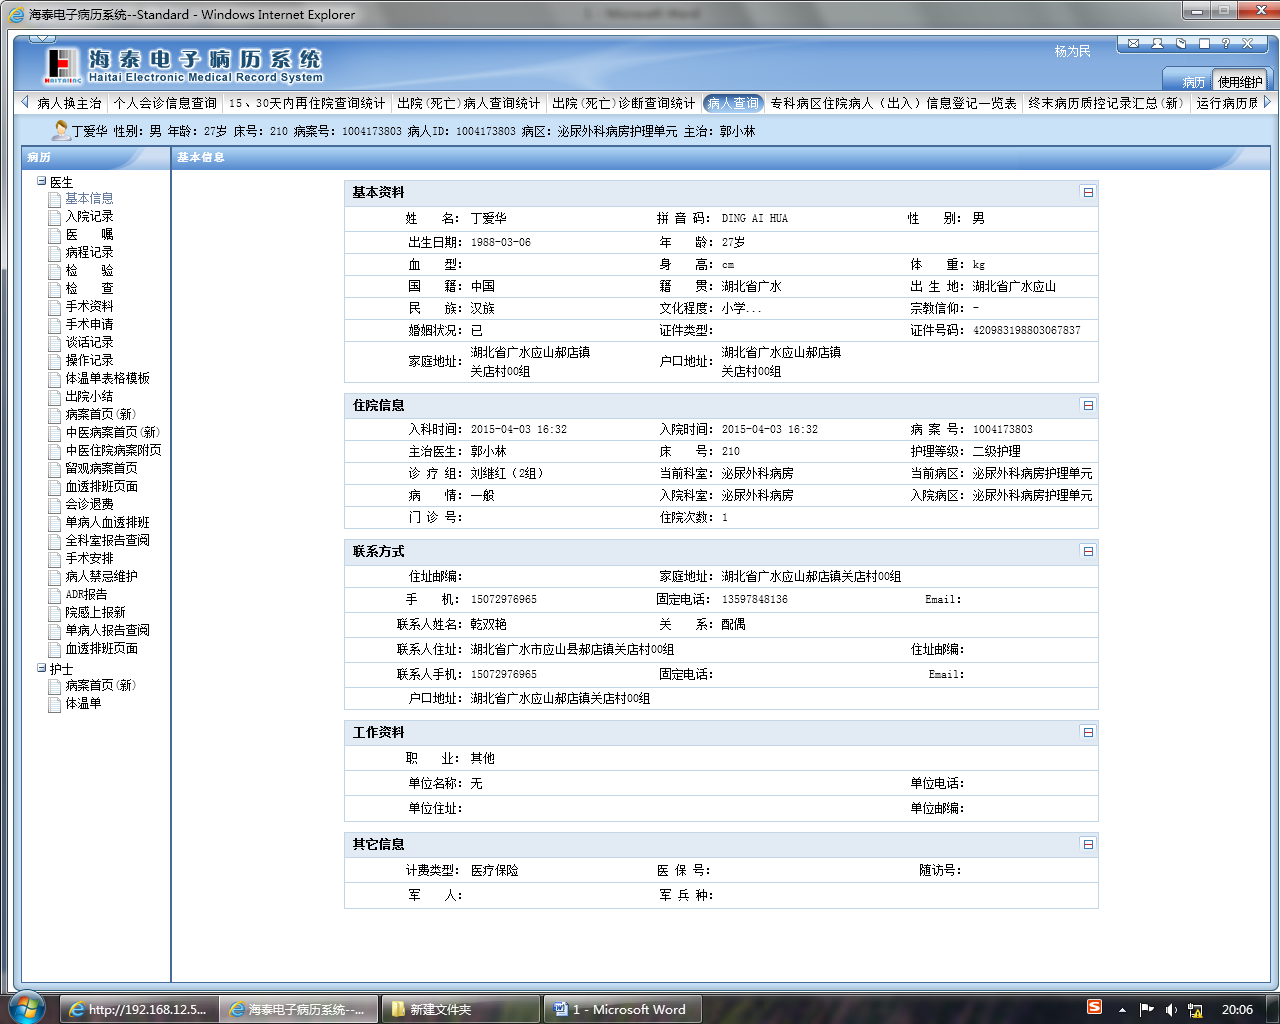
\includegraphics[width=0.9\textwidth]{input-image-1}
	%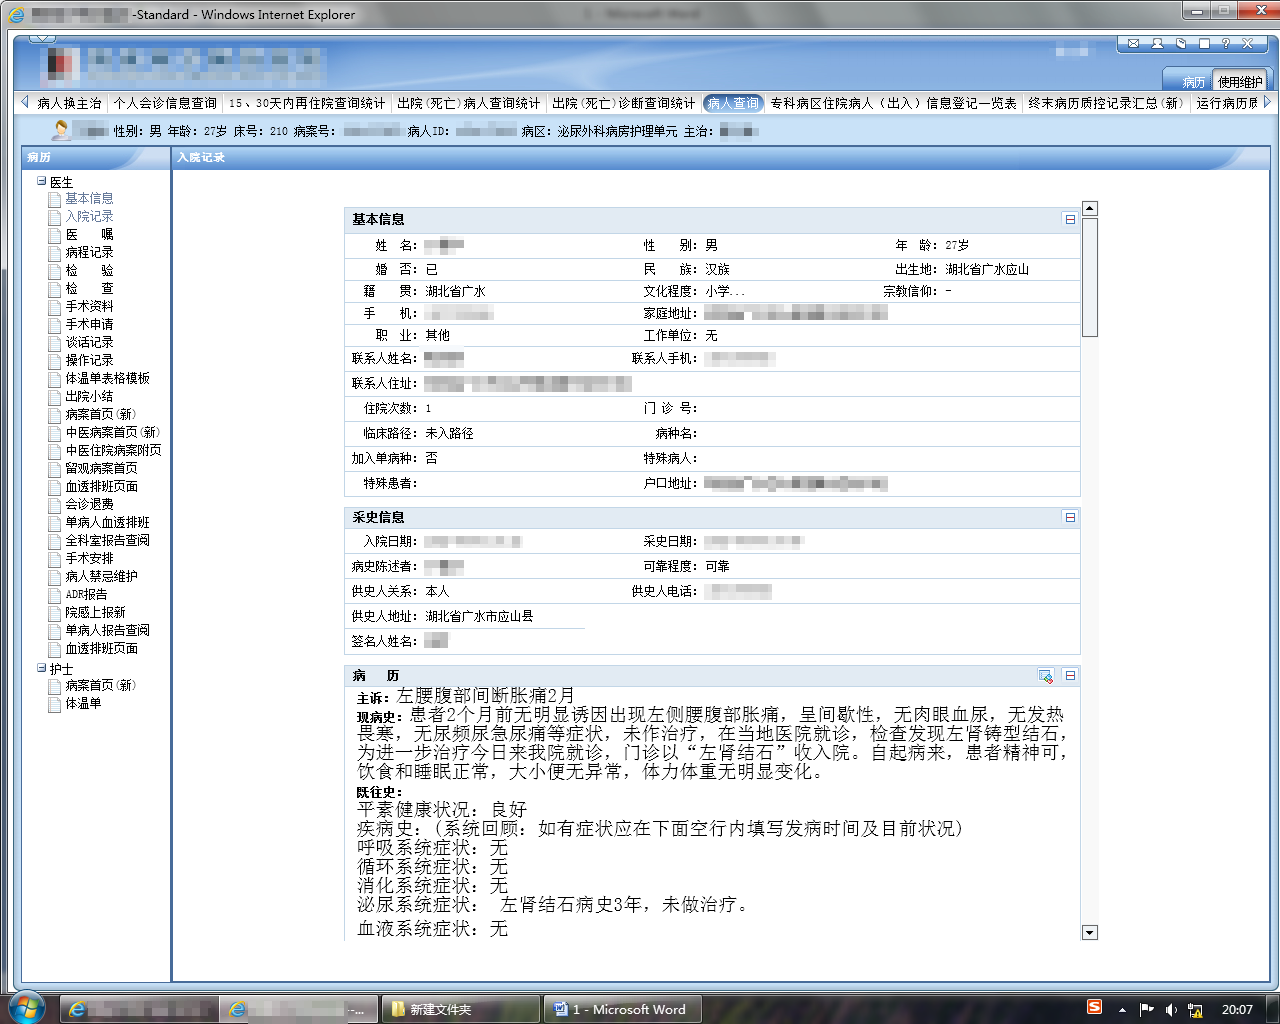
\includegraphics[width=0.48\textwidth]{input-image-2}
	\caption{典型的图片输入数据}
	\label{pic:input-image-1}
\end{figure}

\subsection{输出数据}
医院作为需求方,期望的输出数据是怎样的呢?首先,输出的数据要有一个确定的组织形式(如各个字段之间的序是确定的),这样才能方便系统的下游继续处理,如数据提取、展示、入库等,这一点是不言自明的;与此同时,输出数据也应该有一定的便于展示的属性,何为“便于展示”呢,举个例子,如果输出是一个有序的纯文本数据,它虽然可以符合下游的处理要求,但是本身对于一个普通人来说,是不可读的,而如果输出是一个类似excel的文档,它不仅能交给下游继续处理,也可以直接用个人电脑的excel程序打开浏览,我们称之为其有“便于展示”的属性,显然,excel文档相较于纯文本文档,是一个更符合需求的产出格式。

\subsection{系统性能}
作为一个识别系统,其性能指标的衡量有多个维度,常见的有识别准确性、处理速度、数据吞吐能力以及能效等多方面。其中最为重要的是识别准确率,对于医学档案的识别工作更是如此,因为它的识别牵涉到病人病情的诊断,稍有闪失就可能造成严重后果。因此,系统首先要保证的是识别准确率,相比较而言,处理速度、数据吞吐能力以及能效等,都可以作为次要指标。一般来说,系统需要保证识别的整体准确率应在90\%以上,这里的准确率,既包括版面分析时,字段划分的准确率,也包括后续文本识别的准确率。处理速度上,要保证在单机情况下,处理一份病历数据(一般包含7到10张图片),从图片读取到档案生成产出,要能在3分钟以内完成。

\section{小结}
根据上面的需求分析,整个系统应该满足如下需求:
\begin{itemize}
	\item 输入数据:多张图片组成的病人病历数据。
	\item 输出数据:具有确定数据组织结构的、具备一定可读性的病人病历档案。
	\item 版面分析:系统应能自动判断多张图片的版面,并提取出所需的字段。
	\item 准确率:版面分析和文字识别的准确率要达到90\%以上
	\item 速度:处理一份病历数据(一般包含7到10张图片),从图片读取到档案生成产出,要能在3分钟以内完成。
\end{itemize}
